% This version of CVPR template is provided by Ming-Ming Cheng.
% Please leave an issue if you found a bug:
% https://github.com/MCG-NKU/CVPR_Template.

% \documentclass[review]{cvpr}
\documentclass[final]{cvpr}

\usepackage{times}
\usepackage{epsfig}
\usepackage{graphicx}
\usepackage{amsmath}
\usepackage{amssymb}
\usepackage{multirow}

% Include other packages here, before hyperref.
\usepackage{caption}
\usepackage[tablename=Table]{caption} 
\captionsetup[table]{skip=5pt}
\captionsetup{labelfont=bf}
% If you comment hyperref and then uncomment it, you should delete
% egpaper.aux before re-running latex.  (Or just hit 'q' on the first latex
% run, let it finish, and you should be clear).
\usepackage[pagebackref=true,breaklinks=true,colorlinks,bookmarks=false]{hyperref}


\def\cvprPaperID{****} % *** Enter the CVPR Paper ID here
\def\confYear{CVPR 2021}
%\setcounter{page}{4321} % For final version only


\begin{document}

%%%%%%%%% TITLE
\title{Extraction of individual instrument sound from music file}

\author{Alex Zongo\\
2021280358\\
{\tt\small alexanicetzongo@gmail.com}
% For a paper whose authors are all at the same institution,
% omit the following lines up until the closing ``}''.
% Additional authors and addresses can be added with ``\and'',
% just like the second author.
% To save space, use either the email address or home page, not both
\and
Teiichi Atsuya\\
student id\\
{\tt\small teiichi.atsuya@outlook.com}
\and
Picard Armand\\
2021400607\\
{\tt\small armandpicard71@gmail.com}
}

\maketitle


%%%%%%%%% ABSTRACT
\begin{abstract}
Here is our abstract
\end{abstract}

%%%%%%%%% BODY TEXT
\section{Introduction}

Music we listen to everyday are usually the product of sophisticated work of multi-track editing, the combination of multiple instruments and vocals. 

The question of wether we can reverse-engineer this process by extracting the individual or particular instrument(s) or vocals, out of the entire music has been studied for a while now. Until recently sound source separation was very difficult for many experts who tried to apply their domain knowledge, such as knowledge of the mixing process, with limited applications and sub-optimal sound quality. 

However, with the recent development of deep neural network technology, the AI system is capable of distinguishing the specific frequency and sound of particular instrument(s), such as Drums and Vocals. 

Encouraged by the results of recent studies in this field, we decided to study the different approaches for such task, then pick a model or architecture and try to improve it and finally annotate the results and compare them with existing models under similar experiment settings.


\section{Related work}

In this section we will describe different approaches and model architecture to implement instrument sound extraction using Deep Learning.

\subsection{Different Approaches}
\subsubsection{Waveform}

This type of model takes the raw wave as input. This gives the model all the information available to build it's own representation of the data.
 
Indeed, without any preprocessing, such network intends to capture the frequencies and phase of the wave input and model the sources. A pioneer is Wave-U-Net \cite{waveunet} which inspired new state of art model such Demucs \cite{defossez2019music}, DPTNet \cite{dptnet}, MMDenseLSTM \cite{mm_dense_lstm} and many more.

Since a musical sound usually has a high frequency. Hence, for predictions on a fairly long time period, the model will have a huge number of inputs leading to several operations in a single pass and also expensive in terms of memory consumption, for instance to record the gradients which could exceed the memory of the available resources.
These considerations conditioned our research. 

\subsubsection{Spectrogram}

Spectrogram model take the spectrogram of the audio as input.
To get the spectrogram, Short Time Fourier Transform(STFT) is use.
Then the DeepLearning model is given as input only the magnitude of the spectrogram and it train to produce the magnitude of the different source.
Then to get the final output we reintegrate the phase of the input signal and apply Inverse Short Time Fourier Transform(ISTFT) to get the output audio.

This approach allows the model to have higher level features as input and reduced length depending on the window size and the hop length while doing the STFT.
This higher level features can allow the model to learn faster and being smaller but it also don't give all the information on small local perturbation that can be useful to produce the best final output.



\subsubsection{Hybrid}
The Hybrid approach is mostly used nowadays. Such network has 2 types of input, one for the waveform and one for the spectrogram.  
This allows to have the best of both world by complementing the information extracted from both representations. However it requires a lot of computing power. Example of this kind of model include HybridDemucs \cite{hybrid-demucs} and CatNet \cite{catnet}.

\subsection{Baseline Architecture}

Our baseline model architecture is based on Wave-U-Net. This model use an encoder that down-samples at each step and then a decoder that up-samples the bottleneck using the result of each previous encoder as a second input.
The global architecture of Wave-U-Net\cite{waveunet} is show in Figure~\ref{waveunet-architecture}

\begin{figure}
   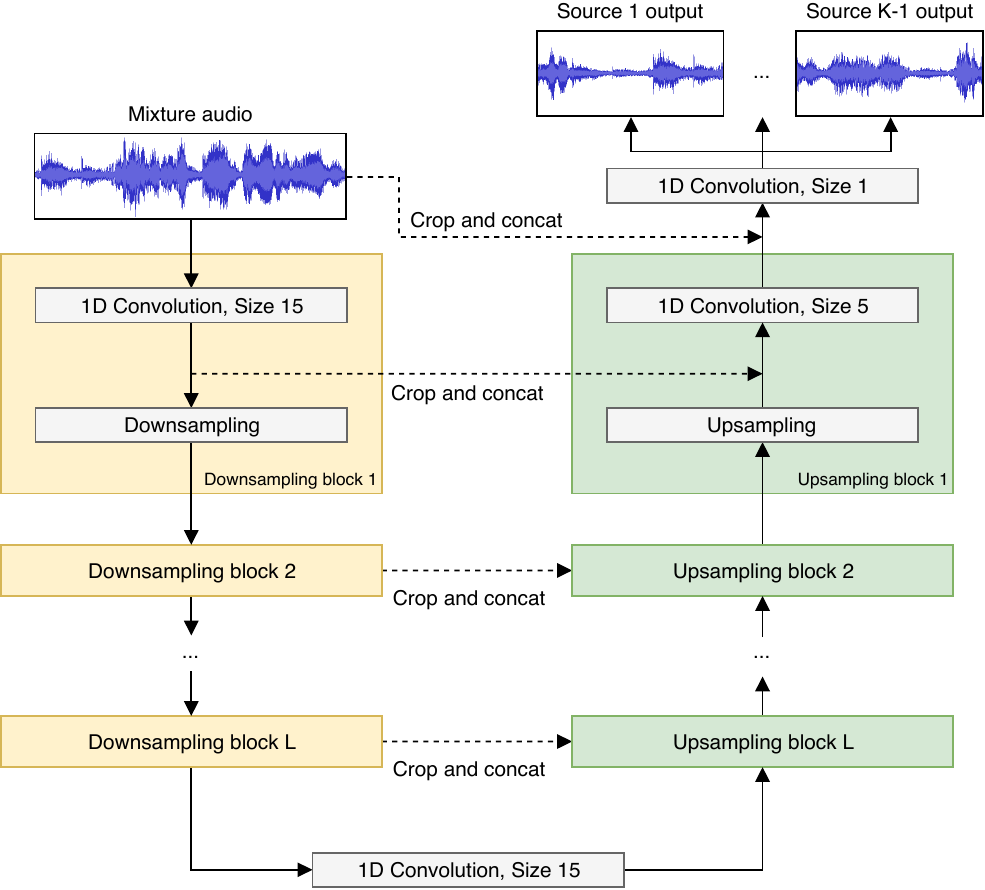
\includegraphics[scale=0.25]{waveunet.png}
   \caption{Wave-U-Net architecture}
   \label{waveunet-architecture}
\end{figure}

\section{Approach}

\subsection{Problem Description}
Our approach consisted in sound separation in the waveform domain. Each sound, here a recording, is a mixture of individual stems, also called sources, regrouped into 4 categories: (1) drums, (2) bass, (3) other, (4) vocals. Each source is a set of sampled frequencies and is represented by a waveform $s_i$ $\epsilon$ ${[-1, 1]}^{C,T}$ where C is the number of channels (here 2 for stereo) and T the number of samples. By defining $\emph{S}:= (s_i)_i$ the concatenation of the sources in a tensor of size (4, C=2, T) and the mixture $M:= \sum^4_{i=1} {s_i}$, the model was trained to minimize
\begin{equation}
\min_{\theta} \sum_{M \epsilon D} l(f_{\theta}(M), S)
\end{equation}
for some dataset $D$, the reconstruction error $l$ (here Mean square error), the model architecture $f$ with one outputs $f$ as a concatenation of the estimated sources $\hat{S}:=f_{\theta}(M):=({\hat{s}_i})_i$ and model weights $\theta$ $\epsilon$ $R^{d}$.

\subsection{Architecture}

\begin{figure}
   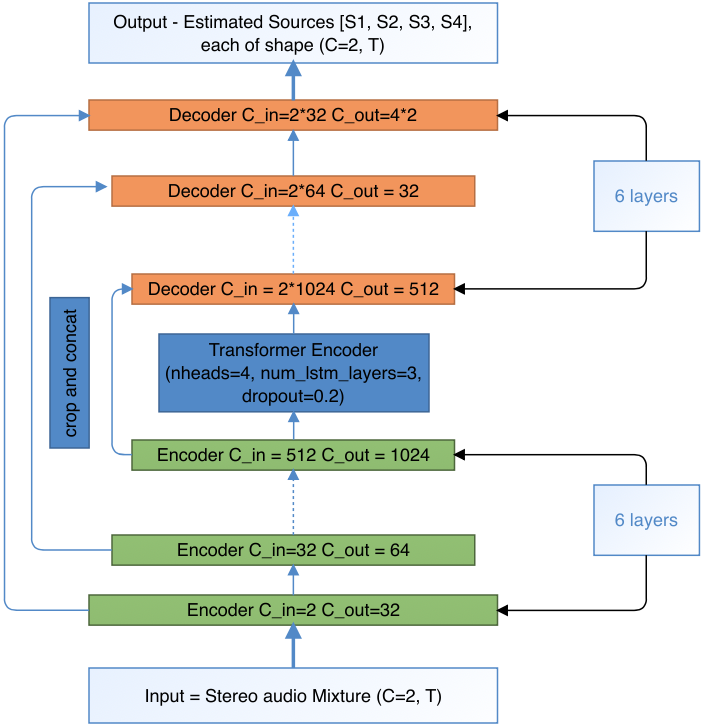
\includegraphics[scale=0.3]{architecture.png}
   \caption{Our model architecture}
   \label{our-architecture}
\end{figure}

The architecture used for the task was developed from a blend ideas between the Wave-U-Net \cite{waveunet} and Demucs \cite{defossez2019music} architectures and the Transformer Encoder from DPTNet\cite{dptnet}.
Basically we used the Wave-U-Net \cite{waveunet} architecture with some modifications in the downsampling layers (encoders), bottlenecks and upsampling layers (decoders).
The network has 6 levels. The encoder and decoder are linked with skipped U-net connections as shown in figure \ref{our-architecture}. Both encoder and decoder include a resampling layer as in \cite{waveunet} for a trainable low-pass filter of fixed size (21). 

The encoder in fig. \ref{encoder} is composed of 6 stacked layers numbered from 1 to 6. $Layer_i$ consists of a pre-shortcut sublayer and a post-shortcut sublayer. The Pre-shortcut sublayer is composed of a convolution with kernel size 5 and stride 1, followed by a group norm with fixed group size of 8, a ReLU activation function, another convolution with kernel size 1 and stride 1 followed by a GLU layer. The post-shortcut sublayer has exactly the same structure as the pre-shortcut sublayer. Both sublayers are separated by the resampling layer \cite{waveunet} with trainable sinc filter of size 21 and with stride 4.

\begin{figure}
   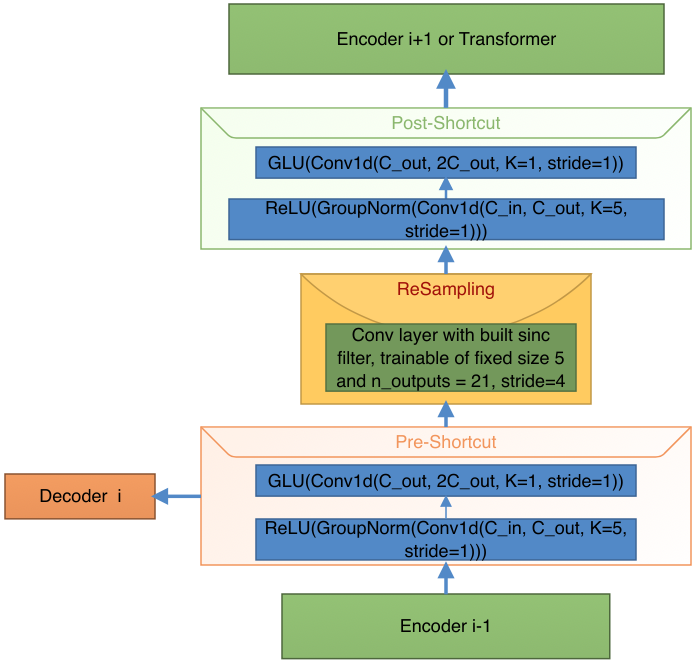
\includegraphics[scale=0.3]{encoder.png}
   \caption{A detail overview of the internal structure of the encoder}
   \label{encoder}
\end{figure}

\begin{figure}
   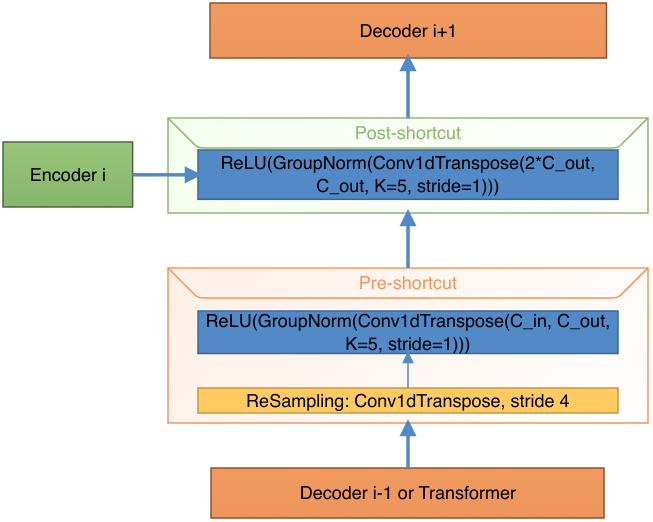
\includegraphics[scale=0.3]{decoder.png}
   \caption{A detail overview of the internal structure of the decoder}
   \label{decoder}
\end{figure}

\begin{figure}
   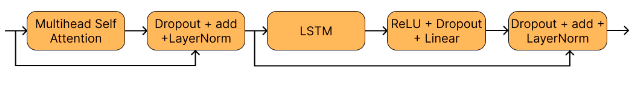
\includegraphics[scale=0.4]{transformer.png}
   \caption{A overview of the transformer encoder}
   \label{transformer}
\end{figure}
The bottleneck is a single transformer encoder (fig. \ref{transformer}) derived from DPTNet\cite{dptnet} with 4 heads, 3 LSTM layers and a dropout of 0.2.


The decoder in fig. \ref{decoder} is almost symmetric to the encoder. In fact it is composed of 6 layers numbered in reverse order. Each layer is also composed of a pre-shortcut and a post-shortcut sublayer. The pre-shortcut layer is preceded by a resampling layer similar to the encoder but with transposed convolution \cite{waveunet}, then a transposed convolution of kernel size 5 and stride 1 followed by a group norm and a ReLU activation function. The post-shortcut consists of a transposed convolution with a doubled input channel because of the coming input from the encoder and a kernel size of 5 with stride 1, a group norm and a ReLU activation function.
The last decoder or final layer is a convolution of kernel size 5 and stride 1, without activation function, which outputs a concatenation of the stereo estimated sources (each with 2 channels).
% cite the paper DPTNet

\section{Experiments and Results}
 The implemented model was evaluated on music separation with bass, drums, vocals and "other" instruments as categories defined by the SiSec Separation campaign \cite{SiSec}.
\subsection{Datasets}
The datasets used was MusDB18-HQ \cite{MUSDB18HQ} as well as MusDB18 7s \cite{musdb18}. Both datasets contain 150 tracks split into 2 subsets. From the 100 songs reserved for training, 25 were dedicated for validation, also used for early stop in training. The remaining 50 were used as test data. The model is fully trained on MusDB18-hq which is stereophonic and encoded at 44.1kHz. The model is then evaluated on both datasets.
Data augmentation is also performed on the training data by multiplying the sources of the mixture with a uniformly chosen factor between 0.7 and 1.0 and then summing the resulting sources back to obtain a new mixture.\cite{waveunet}  
\subsection{Training Procedure}
During training, one epoch was defined as a pass over 3 seconds extracts on the data with a batch size of 8. The inputs were padded accordingly to ensure input context and alleviate bottlenecks. Furthermore, we use the mean square loss (MSE) over all source output samples in a batch. The optimizer was ADAM with a cyclic learning [$1*10^{-3}$, $5*10^{-5}$]. 

The model was trained with early stopping after 20 epochs with no improvement on the validation dataset by the MSE loss. Afterwards, the model is fined with a cyclic learning [$5*10^{-4}$, $5*10^{-6}$], until 50~100 epochs with no improvements validation loss. The best model on validation loss was then selected and used on the test set. 

Experiments were also performed on the number of levels (depth) of the network, the output size, the kernel or filter sizes as well as structures such as LSTMs and fully connected layers as bottleneck layers to arrive at a better model with transformers.   
\subsection{Model Settings}
The model uses at least 137897 inputs and 132441 outputs based on the valid convolutions. Besides all the tracks are sampled at 44.1kHz. The model has 12 layers and the transformer encoder as bottleneck. The number of filter for the resampling both in encoder and decoder were fixed to 21.
\subsection{Evaluation Metrics}
The metric commonly used to evaluate sound source separation performance is the Signal-to-Distortion Ratio (SDR) \cite{sdr}. Indeed, a track is partitioned into non-overlapping audio segments multiple seconds in length, and segment-wise metrics are then averaged over each audio track or the whole dataset to evaluate the model. We use the python package \emph{museval}\footnote{\url{https://github.com/sigsep/sigsep-mus-eval}} which provides a reference implementation for the SiSec Mus 2018 campaign \cite{SiSec}.

If we reuse the notations from \cite{sdr}, let's take a source $j$ $\epsilon$ $1, 2, 3, 4$ and we introduce $P_{s_{j}}$ the orthogonal projection on $s_{j}$ and $P_{s}$ the projection on the Span($s_{1}$, \dots, $s_{4}$). By taking the estimate of source $s_{j}$, $s_{target}:=P_{s_j}(s_j)$, $e_{interference}:=P_s(s_j)-P_{s_j}(s_j)$ and $e_{artifact}:=s_j-P_s(s_j)$,
the SDR is defined as
\begin{equation}
   SDR = 10\log_{10} \frac{||s_{target}||^2}{||e_{interference}+e_{artifact}||^2}
\end{equation}
One the drawbacks of such formula is the undefined results ($\log(0)$) when the source is silent or nearly silent as pointed out in \cite{waveunet}. Indeed the SDR is very low when the output is quiet. Such outliers encountered affect the overall evaluation because of the average over all segments. Hence as done in \cite{SiSec}, we report the median over all tracks of the median of the metric over each track. This ensure robustness and describes the minimum performance achieved $50\%$ of the time.  
\subsection{Results}
The results shown here (see table \ref{dataset-sdr}) are of the best model obtained so far at the end of the experiments. Moreover, we compare our results to state of art performances on the same task under the same datasets.
Table \ref{wave-unet-vs-our-model} indicates an overall improvement of our model which exceeds the performance of Wave-U-Net on the MusDB18-HQ. The main difference between the two models is the transformer encoder that replaced the convolutional bottleneck in Wave-U-Net. Such implementation added some kind of memory to the network, which proves the importance of relation of subsequent frequencies or musical notes in a melody in the separation.

Table \ref{demucs-vs-our-model} on the other shows that our model still has a long way to go. In fact Demucs\cite{defossez2019music} consists in a direct synthesis. The main benefit of synthesis is that we can use a relatively large stride in the decoder, thus speeding up the computations and allowing for a larger number of channels.This explains the effectiveness of the Demucs network, while our model as well as Wave-U-Net \cite{waveunet}, generates its output by iteratively upsampling, adding back the high frequency part of the signal from the matching encoder output (or from the input for the last decoder layer) and filtering.

Table \ref{efficiency-parameters} compares our model to Wave-U-Net and Demucs in terms of parameters and computations. In fact, the developed model has additional parameters because of the transformer encoder which is not detrimental to the performance. Compared to Demucs \cite{defossez2019music} which has 5 times more parameters, we believe that with more experiments on the use of transformer in the model architecture, meaning adding memory in U-Net based models, as well as extra-data as in \cite{hybrid-demucs}  interesting outcomes are expected. 



\begin{table}[]
   \begin{tabular}{|l|ll|ll|}
   \hline
                                                                 & \multicolumn{2}{c|}{Training Set}                    & \multicolumn{2}{c|}{Test Set}                        \\ \hline
                                                                 & \multicolumn{1}{l|}{\begin{tabular}[c]{@{}l@{}}MSE \\ loss\end{tabular}}        & \begin{tabular}[c]{@{}l@{}}Overall\\ SDR \end{tabular}  & \multicolumn{1}{l|}{\begin{tabular}[c]{@{}l@{}}MSE \\ loss\end{tabular}}        & \begin{tabular}[c]{@{}l@{}}Overall\\ SDR \end{tabular}   \\ \hline
   \begin{tabular}[c]{@{}l@{}}MusDB18 \\ 7s dataset\end{tabular} & \multicolumn{1}{l|}{0.0009}          & 6.31          & \multicolumn{1}{l|}{0.0019}          & \textbf{3.41} \\ \hline
   MusDB18-hq                                                    & \multicolumn{1}{l|}{\textbf{0.0005}} & \textbf{6.48} & \multicolumn{1}{l|}{\textbf{0.0016}} & 3.30          \\ \hline
   \end{tabular}

   \caption{Performance of our model on training set and test set in terms of Signal-to-distortion ratio. The higher SDR for MusDB18-hq is explained by the huge number of 
   samples compared to MusDB18 7s which has only 7s extracts from the original songs.}
   \label{dataset-sdr}
\end{table}


\begin{table}[]
   \begin{tabular}{|l|lllll|}
   \hline
   Architectures & \multicolumn{5}{c|}{SDR in dB on Test Set}                                                                                                                        \\ \hline
                 & \multicolumn{1}{l|}{All}           & \multicolumn{1}{l|}{bass}          & \multicolumn{1}{l|}{drums}         & \multicolumn{1}{l|}{other}         & vocals        \\ \hline
   Wave-U-Net    & \multicolumn{1}{l|}{3.17}          & \multicolumn{1}{l|}{\textbf{3.17}} & \multicolumn{1}{l|}{4.16}          & \multicolumn{1}{l|}{2.24}          & 3.05          \\ \hline
   Our Model     & \multicolumn{1}{l|}{\textbf{3.30}} & \multicolumn{1}{l|}{2.91}          & \multicolumn{1}{l|}{\textbf{4.26}} & \multicolumn{1}{l|}{\textbf{2.43}} & \textbf{3.70} \\ \hline
   \end{tabular}
   
   \caption{Comparison of Wave-U-Net and Our model on waveform data (MusDB18)}
   \label{wave-unet-vs-our-model}
\end{table}

\begin{table}[]
   \begin{tabular}{|l|lllll|}
   \hline
   Architectures & \multicolumn{5}{c|}{SDR in dB on Test Set}                                                                                                                        \\ \hline
                 & \multicolumn{1}{l|}{All}           & \multicolumn{1}{l|}{bass}          & \multicolumn{1}{l|}{drums}         & \multicolumn{1}{l|}{other}         & vocals        \\ \hline
   Demucs        & \multicolumn{1}{l|}{\textbf{4.81}} & \multicolumn{1}{l|}{\textbf{5.07}} & \multicolumn{1}{l|}{\textbf{5.38}} & \multicolumn{1}{l|}{\textbf{3.01}} & \textbf{5.44} \\ \hline
   Our model     & \multicolumn{1}{l|}{3.30}          & \multicolumn{1}{l|}{2.91}          & \multicolumn{1}{l|}{4.26}          & \multicolumn{1}{l|}{2.43}          & 3.70          \\ \hline
   \end{tabular}
   \caption{Comparison of Demucs and Our model on waveform data (MusDB18) with no-extra data }
   \label{demucs-vs-our-model}
\end{table}

\begin{table}[]
   \begin{tabular}{|l|l|l|l|l|}
   \hline
   \textbf{Model}      & \textbf{Structure}                                                       & \textbf{Dataset} & \textbf{\begin{tabular}[c]{@{}l@{}} \# $10^6$ of \\ params\end{tabular}} & \textbf{\begin{tabular}[c]{@{}l@{}}GMACs\end{tabular}} \\ \hline
   \textbf{Demucs}     & \begin{tabular}[c]{@{}l@{}}Encoder-\\ LSTM-\\ Decoder\end{tabular}          & \begin{tabular}[c]{@{}l@{}} 150 \\ tracks\end{tabular}       & 415.09                                                                                 & 5.17                                                                            \\ \hline
   \textbf{Wave-U-Net} & \begin{tabular}[c]{@{}l@{}}Encoder-\\ Conv-\\ Decoder\end{tabular}          & \begin{tabular}[c]{@{}l@{}} 150 \\ tracks\end{tabular}       & \textbf{70,15}                                                                         & 98.64                                                                           \\ \hline
   \textbf{Our model}  & \begin{tabular}[c]{@{}l@{}}Encoder-\\ Transformer- \\ -Decoder\end{tabular} & \begin{tabular}[c]{@{}l@{}} 150 \\ tracks\end{tabular}      & 89.27                                                                                  & 40.54                                                                           \\ \hline
   \end{tabular}
   \caption{Our model has more parameters compared to Wave-U-Net mainly because of the transformer encoder. However, it more more efficient since the sources are modeled jointly and separated only in the last layer.  }
   \label{efficiency-parameters}
   \end{table}

\section*{Discussion and Conclusion}
In this paper, we developed a modified version of Wave-U-Net for an end-to-end audio source separation without pre- or post-processing. The idea was not to outperform existing state of the art models but to experiment with the deep learning architectures learned in class to build a lighter model (fewer parameters) which would still capable of reaching reasonable results. The experimental results showed that the model outperformed the Wave-U-Net \cite{waveunet} under comparable settings with our limited data and computing resources. The novelty resides in the inclusion of transformer in the architecture which we believe, is mainly responsible of the efficiency of the model.

However, Demucs \cite{defossez2019music} as well as its hybrid version \cite{hybrid-demucs} exceeds the performance of our model. For future studies, in addition to extra data, new loss function besides MSE to appropriately perceive the loss of quality as indicated in \cite{waveunet}, as well as the extension of pur model to spectral analysis as in \cite{hybrid-demucs}, transformers as in \cite{dptnet} seem to bring some value and its worth investigating.   
{\small
\bibliographystyle{ieee_fullname}
\bibliography{egbib}
}

\end{document}
